\documentclass{article}
\usepackage{graphicx} % Required for inserting images
\usepackage{listings}
\usepackage{minted}
\usepackage[margin=3cm]{geometry}




\begin{document}
\begin{titlepage}
    \begin{center}
        
\includegraphics[width=0.25\textwidth]{PROTECO.png}\hfill
        \hspace{5cm}
        
\includegraphics[width=0.25\textwidth]{UNAM.png}\\[1cm]
        \vspace{1cm}
        \fontsize{30}{10}\selectfont
        \textbf{PROYECTO}\\
        \vspace{0.5cm}
        \fontsize{25}{10}\selectfont
        \textbf{TERMINAL DE TRABAJO 
        PREBESHELL}\\
        \vspace{1.5cm}
        \fontsize{20}{10}\selectfont
        \textbf{Nombre del autor: Alejandro Cortés Mora}\\
        \vspace{0.5cm}
        \textbf{Nombre del autor: Samuel Moíses Flores Aguirre}\\
        \vspace{0.5cm}
        \large 22 de Abril de 2023\\
        \vspace{1.5cm}
        \vspace{1cm}
        \textbf{Facultad de Ingeniería}\\
        \textbf{Universidad Nacional Autónoma de México}\\
        \vspace{1cm}
    \end{center}
\end{titlepage}


\section{Introducción}
\vspace{0.7cm}

\fontsize{14}{8}\selectfont
\textbf{}
En la actualidad, Linux es uno de los sistemas operativos más utilizados en todo el mundo, especialmente en entornos de desarrollo y servidores. Una de las características más destacadas de Linux es su capacidad para trabajar a través de la línea de comandos, lo que lo hace especialmente atractivo para aquellos que desean trabajar en un entorno más técnico y avanzado.

\vspace{0.5cm}El objetivo de este proyecto es programar e implementar una terminal para diferentes sistemas operativos basados en GNU/linux. Es un proycto que se llevo a cabo como parte de la evaluacion dl curso Linux para los prebecarios, representando asi un reto, ya que consiste en organizar tiempos, trabajar en equipo, aplicar lo aprendido, e investigar por cuenta prpia, propiciando asi un desarrollo integral. La elaboracion se baso en una sistematizacion y organizacion de los tiempos basado en un cronograma que beneficiara a ambas partes. Esta terminal ejecuta comandos como lo son: ayuda, informacion del sistema, creditos, busqueda de archivos en carpetas, la fecha y hora, un juego, y un reproductor de musica. A lo largo de este proyecto se profundizaran en diferentes temas, como lo es manejo de variables, ingreso a direcciones y rutas, ciclos y arreglos. Por lo que al termino de este proyecto se espera un aprendizaje general sobre estos temas previamente mencionados. 

\begin{figure}[h]
  \centering
  
\includegraphics[width=0.5\textwidth]{Linux.png}
\end{figure}


\newpage
\section{Desarrollo}

\subsection{Infosis}
\fontsize{10}{10}\selectfont
\begin{minted} {bash}
#!/bin/bash

echo ""
echo ""
echo -e "\e[34m   _____ _____  _____ _______ ______ __  __           \e[0m"
echo -e "\e[34m  / ____|_   _|/ ____|__   __|  ____|  \/  |   /\     \e[0m"
echo -e "\e[34m | (___   | | | (___    | |  | |__  | \  / |  /  \    \e[0m"
echo -e "\e[34m  \___ \  | |  \___ \   | |  |  __| | |\/| | / /\ \   \e[0m"
echo -e "\e[34m  ____) |_| |_ ____) |  | |  | |____| |  | |/ ____ \  \e[0m"
echo -e "\e[34m |_____/|_____|_____/   |_|  |______|_|  |_/_/    \_\ \e[0m"
echo ""
echo ""

Mem_RAM=$(grep MemTotal /proc/meminfo | awk '{print $2 / 1024}')
echo "Memoria RAM: $Mem_RAM Mb"


SO=$(lsb_release -d | awk '{printf $2 " " $3 " " $4}')
echo "Sistema Operativo: $SO"

Arquitectura=$(lscpu| awk '/Arquitectura/ {print $2}')
echo "Arquitectura: $Arquitectura"
\end{minted}

\begin{center}
    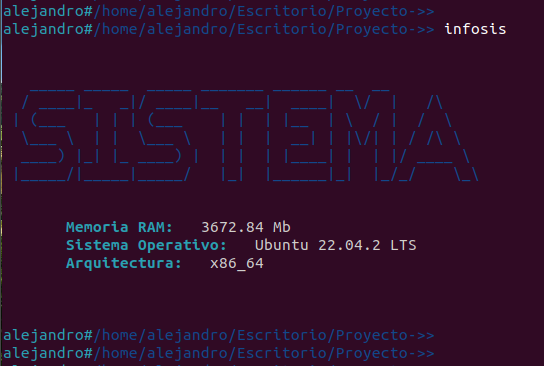
\includegraphics[width=0.7\textwidth]{capturaInfosis.png}
\end{center}

\vspace{1cm}
\fontsize{12}{6}\selectfont
\textbf{}

En este comando se muestra la informacion del sistema operativo en que se ejecuta la terminal, de igual forma, la memoria RAM, y el tipo de arquitectura que usa el dispositivo.
\newpage


\subsection{Buscar}
\fontsize{10}{10}\selectfont
\begin{minted}[language=bash]{sh}
#!/bin/bash

echo -e -n "\e[33mDame el nombre del archivo a buscar: \e[0m"
read archivo

echo -e -n "\e[34mDame la ruta donde vas a buscar el archivo: \e[0m"
read carpeta


if ls "$HOME/$carpeta" | egrep "$archivo"
	then 
	echo -e "\e[32mEl archivo se encontro correctamente \e[0m"
else
	echo -e "\e[31mNo se encontro el archivo \e[0m"
fi
\end{minted}
\vspace{1.5cm}

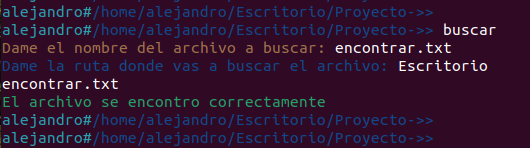
\includegraphics[width=1\textwidth]{campturaBuscar.png}

\vspace{1.5cm}
\fontsize{12}{6}\selectfont
\textbf{}
Este comando permite buscar un archivo de acuerdo a la ruta que especifique el usuario. Primeramente el usuario ingresa el nombre del archivo a buscar y posteriormente la ruta de manera explicita.


\newpage
\subsection{Fecha}
\fontsize{9}{4.5}
\begin{minted}[language=C++]{C++}

# incluir < stdio.h >
# incluir < tiempo.h >

int  principal ()
{
	tiempo_t t;
	tiempo (&t);
	printf ( " %s \n " , ctime (&t));

	struct  tm *tiempo = horalocal (&t);

	printf ( " %d / %d / %d " ,tiempo-> tm_mday , tiempo-> tm_mon + 1 , tiempo-> tm_year + 1900 );
 
	retorno ( 0 );
}

\end{minted}

\begin{minted}[language=sh]{sh}


#! /bin/bash

fecha= $( ./obtener_fecha )

echo  $fecha

\end{minted}

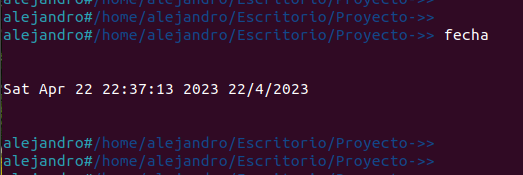
\includegraphics[width=.8\textwidth]{capturaFecha.png}
\vspace{1cm}

\fontsize{12}{6}\selectfont
\textbf{}
Este comando proporciona el dia abreviado en ingles, el mes abreviado en ingles, el dia, la hora con formato Horas : Minutos : Segundos, en formato ampliado de 24 horas, el año, y la fecha en formato abreviado dia / mes / año  


\subsection{Juego de GATO}
\fontsize{7}{10}\selectfont
\begin{minted}{bash}
#!/bin/bash

# Define las variables para el tablero
tablero=(' ' ' ' ' ' ' ' ' ' ' ' ' ' ' ' ' ')
jugador_actual='X'
ganador=false
estatico=(1 2 3 4 5 6 7 8 9)

# Función que dibuja el tablero
function dibujar_tablero {
  echo ""
  echo ""
  echo " ${tablero[0]} | ${tablero[1]} | ${tablero[2]} _______ | ${estatico[0]} | ${estatico[1]} | ${estatico[2]} |"
  echo "---+---+---        +---+---+---+"
  echo " ${tablero[3]} | ${tablero[4]} | ${tablero[5]} _______ | ${estatico[3]} | ${estatico[4]} | ${estatico[5]} |"
  echo "---+---+---        +---+---+---+"
  echo " ${tablero[6]} | ${tablero[7]} | ${tablero[8]} _______ | ${estatico[6]} | ${estatico[7]} | ${estatico[8]} |"
}

# Función que verifica si hay un ganador
function verificar_ganador {
  if [[ ${tablero[0]} != ' ' && ${tablero[0]} == ${tablero[1]} && ${tablero[1]} == ${tablero[2]} ]]; then
    ganador=true
  elif [[ ${tablero[3]} != ' ' && ${tablero[3]} == ${tablero[4]} && ${tablero[4]} == ${tablero[5]} ]]; then
    ganador=true
  elif [[ ${tablero[6]} != ' ' && ${tablero[6]} == ${tablero[7]} && ${tablero[7]} == ${tablero[8]} ]]; then
    ganador=true
  elif [[ ${tablero[0]} != ' ' && ${tablero[0]} == ${tablero[3]} && ${tablero[3]} == ${tablero[6]} ]]; then
    ganador=true
  elif [[ ${tablero[1]} != ' ' && ${tablero[1]} == ${tablero[4]} && ${tablero[4]} == ${tablero[7]} ]]; then
    ganador=true
  elif [[ ${tablero[2]} != ' ' && ${tablero[2]} == ${tablero[5]} && ${tablero[5]} == ${tablero[8]} ]]; then
    ganador=true
  elif [[ ${tablero[0]} != ' ' && ${tablero[0]} == ${tablero[4]} && ${tablero[4]} == ${tablero[8]} ]]; then
    ganador=true
  elif [[ ${tablero[2]} != ' ' && ${tablero[2]} == ${tablero[4]} && ${tablero[4]} == ${tablero[6]} ]]; then
    ganador=true
  fi
}

# Función que solicita la jugada del jugador
function jugar {
  echo "Es el turno del jugador $jugador_actual"
  read -p "Ingrese una posición (1-9): " posicion
  while [[ ${tablero[posicion-1]} != ' ' ]]; do
    read -p "La posición $posicion ya está ocupada. Ingrese otra posición (1-9): " posicion
  done
  tablero[posicion-1]=$jugador_actual
}

# Ciclo del juego
while [[ $ganador == false ]]; do
  dibujar_tablero
  jugar
  verificar_ganador
  if [[ $ganador == true ]]; then
    dibujar_tablero
    echo "¡El jugador $jugador_actual ha ganado!"
    break
  fi
  if [[ ! " ${tablero[@]} " =~ " " ]]; then
    dibujar_tablero
    echo "¡Es un empate!"
    break
  fi

  # Cambia al siguiente jugador
  if [[ $jugador_actual == 'X' ]]; then
    jugador_actual='O'
  else
    jugador_actual='X'
  fi
done
\end{minted}
\begin{center}
    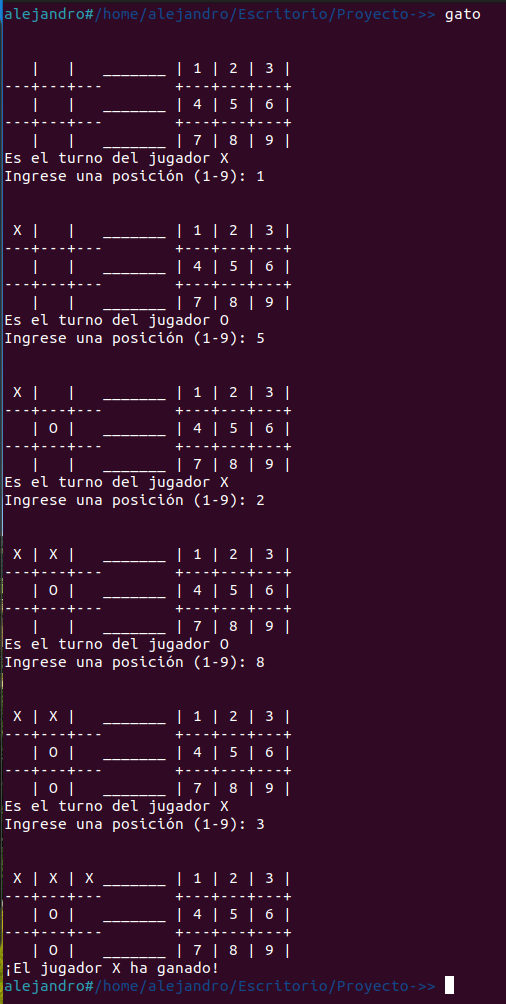
\includegraphics[width=.6\textwidth]{capturaJuego.png}
\end{center}


\vspace{1cm}
\fontsize{12}{6}\selectfont
\textbf{}
Este comando permite ingresar al juego del Gato, se requieren de dos personas para poder jugar, mostrando el simbolo del ganador, se utilizan dos tableros, uno donde se ingresaran los simbolos y otro que será la referencia, mostrara las posiciones donde se pueden colocar los simbolos con números. 


\newpage
\subsection{Reproductor MP3}
\fontsize{6}{4.5}
\begin{minted}[language=bash]{sh}
    #!/bin/bash

function opciones(){
    echo "OPCIONES"
    echo "Presione la tecla:"
    echo "1. Detener la reproducción - Tecla q "
    echo "2. Pausar y reanudar la reproducción -Tecla s"
    echo "3. Bajar volumen - Tecla -"
    echo "4. Subir volumne - Tecla +"
    echo "5. Repetir cancion - Tecla b"

}


echo "Bienvenido al reproductor MP3"


if ! command -v mpg123 &>/dev/null || ! command -v cava &>/dev/null; then
  echo "mpg123 y projectm no se encuentran instalados"
  while true; do
    read -p "¿Desea instalarlo? (s/n): " instalar
    case $instalar in
      [Ss]* )
        
        sudo apt update
        sudo apt install mpg123 cava 
        break
        ;;
      [Nn]* )
        echo "El reproductor MP3 no puede funcionar sin mpg123 y projectm."
        exit
        ;;
      * )
        echo "Ingrese 's' para sí o 'n' para no."
        ;;
    esac
  done
fi

opc=""

while true; do
echo "¿Cómo desea escuchar su música?" 
echo "Seleccione una opción:"
echo "1. Reproducir una canción"
echo "2. Reproducir un repertorio de canciones"
echo "3. Reproducir canciones de manera aleatoria"

read opc

case $opc in

"1")
    echo "Seleccione la ruta de su canción"
    while true; do
      read -p "Ingrese la ruta del archivo MP3 o 'q' para salir: " archivo
      if [ "$archivo" == "q" ]; then
        echo "Saliendo..."
        break
      fi
      archivo=$(echo "$archivo" | sed "s/'//g")
      if [ -f "$archivo" ]; then
        opciones
        gnome-terminal --tab --title="cava" -- bash -c "cava; exec bash"
        mpg123 "$archivo"
      else
        echo "Por favor, ingrese una ruta válida."
      fi
    done
    ;;

"2")
    echo "Seleccione la ruta de su repertorio"
    while true; do
      read -p "Ingrese la ruta del repertorio o 'q' para salir: " archivo
      if [ "$archivo" == "q" ]; then
        echo "Saliendo..."
        break
      fi
      archivo=$(echo "$archivo" | sed "s/'//g")
      if [ -d "$archivo" ]; then
          opciones
          echo "6. Reproducir siguiente canción - Tecla f"
          echo "7. Reproducir canción anterior - Tecla d"
          mpg123 "$archivo"/*.mp3
        
      else
        echo "Ruta incorrecta, ingrese una ruta válida."
      fi
    done
    ;;

"3")
    echo "Seleccione la ruta de su repertorio"
    while true; do
      read -p "Ingrese la ruta del repertorio o 'q' para salir: " archivo
      if [ "$archivo" == "q" ]; then
        echo "Saliendo..."
        break
      fi
      archivo=$(echo "$archivo" | sed "s/'//g")
      if [ -d "$archivo" ]; then
        mpg123 -z "$archivo"/*.mp3
        opciones
        echo "3. Reproducir siguiente canción - Tecla f"
        echo "4. Reproducir canción anterior - Tecla d"
      else
        echo "Ruta incorrecta, ingrese una ruta válida."
      fi
    done
    ;;
esac
done

\end{minted}

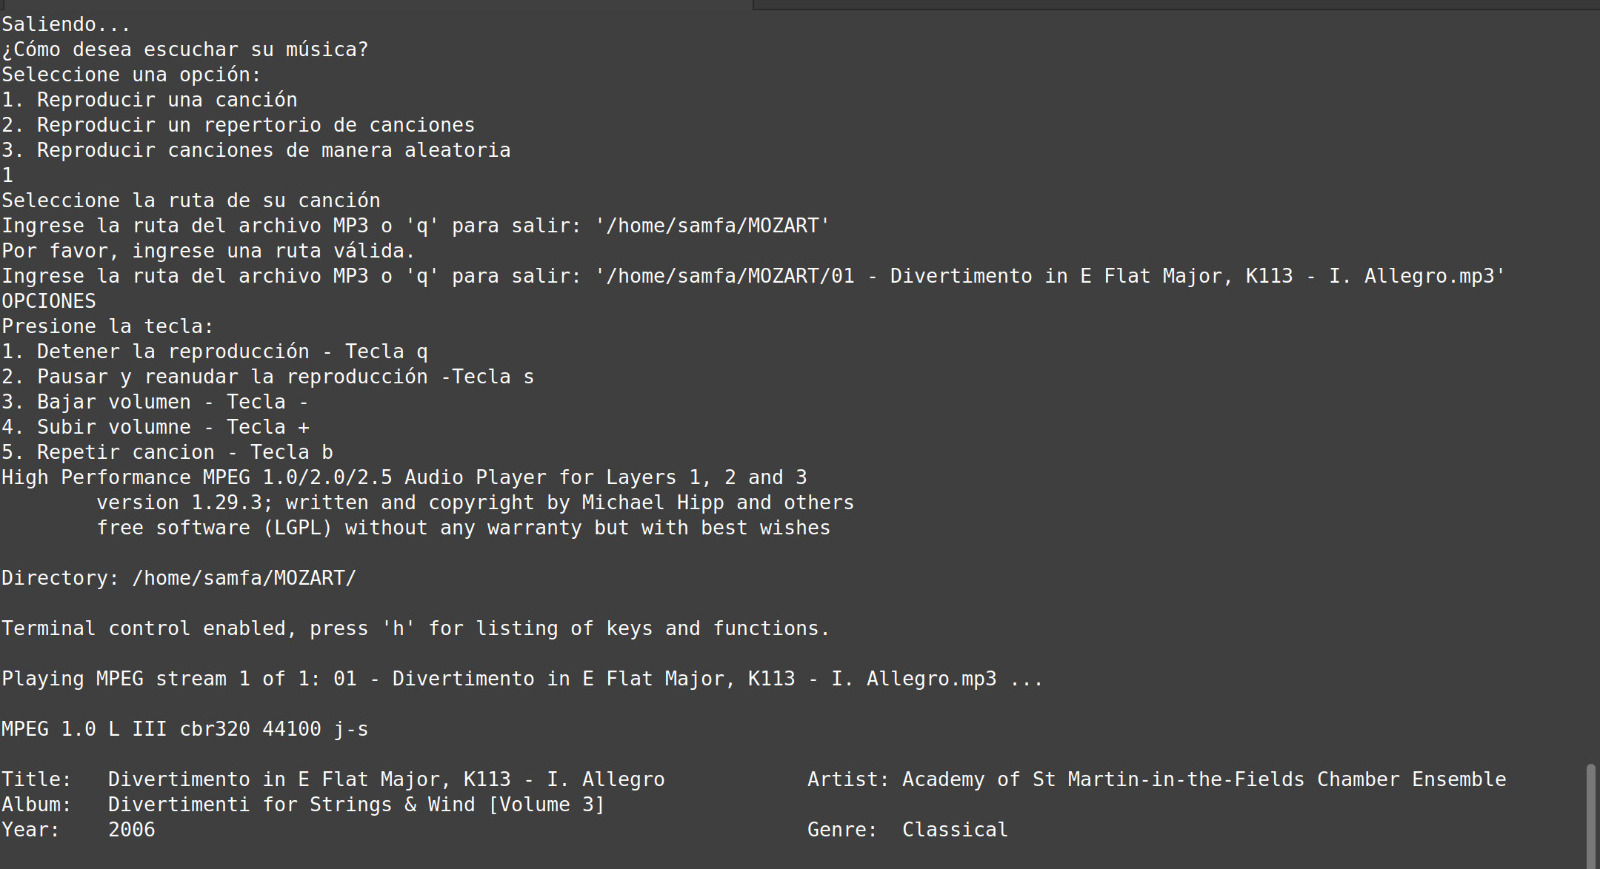
\includegraphics[width=1\textwidth]{capturaReproductor1.jpeg}

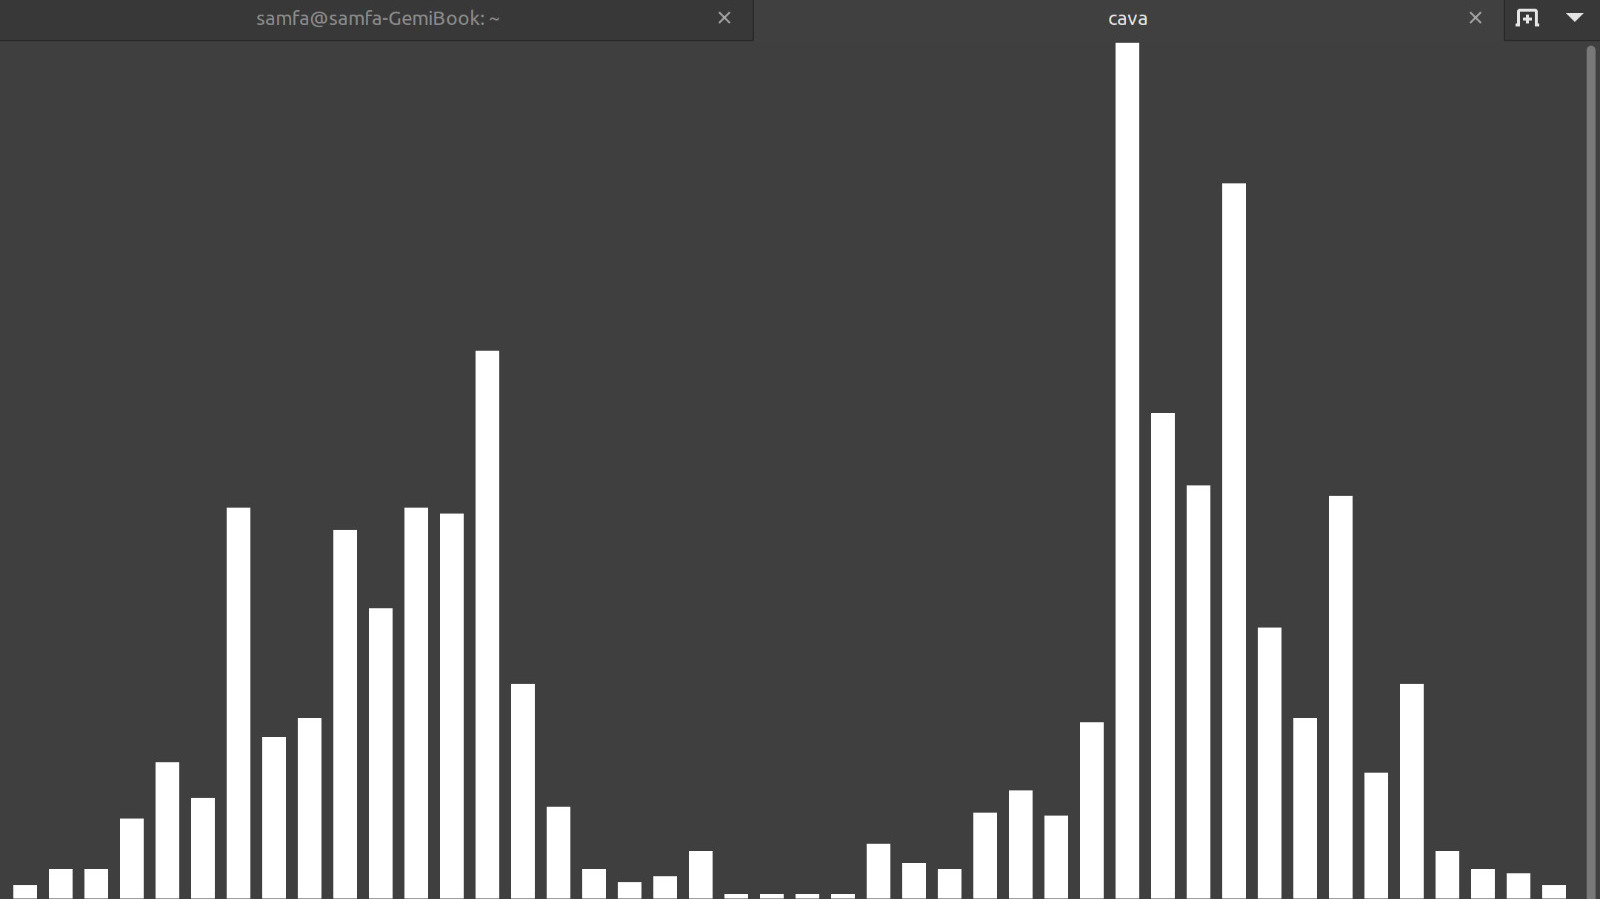
\includegraphics[width=1\textwidth]{capturaReproductor2.jpeg}

\vspace{1cm}
\fontsize{12}{6}\selectfont
\textbf{}

Este comando permite reproducir una cancion en formato mp3, asi como algun repertorio o carpeta en la que un usuario almacene una gran cantidad de canciones. Por medio de mpg123 se realizan algunas funciones basicas como repetir la cancion, reproducir la siguiente cancion, pausar la reproduccion, quitar la cancion, entre otras. Ademas de contar con un visualizador.

\newpage
\subsection{Ayuda}
\fontsize{4}{4.5}\selectfont
\begin{minted}[language=bash]{sh}

#!/bin/bash
echo ""
echo ""
echo ""

echo "     |7|7|7|      \7\     /7/   |7|7|    |7|7|  |7|7|7|7|7\           |7|7|7|       " 
echo "    /7/    \7\     \7\   /7/    |7|7|    |7|7|  |7|7|     \7\        /7/    \7\     "
echo "   /7/  __  \7\     \7\ /7/     |7|7|    |7|7|  |7|7|     \7\7\     /7/  __  \7\   "
echo "  /7/  /  \  \7\     |7|7|      |7|7|    |7|7|  |7|7|     \7\7\    /7/  /  \  \7\  "
echo " /7/  /____\  \7\    |7|7|      \7\7\    /7/7/  |7|7|     \7\     /7/  /____\  \7\  "
echo "/7/            \7\   |7|7|        |7|7|7|7|7|   |7|7|7|7|7\      /7/            \7\ "

echo ""
echo ""
echo ""
echo ""
echo -e "\e[1;35m             -> ayuda       \e[0m    \e[36;4mProporciona un listado de comandos, con una brebe descripcion, que el usuario puede ejecutar \e[0m"

echo ""
echo ""
echo -e "\e[1;35m             -> infosis     \e[0m    \e[36;4mMuestra la informacion del sistema operativo: \e[1mMemoria RAM, Version del SO, Arquitectura del Sistema \e[0m \e[0m"

echo ""
echo ""
echo -e "\e[1;35m             -> fecha       \e[0m    \e[36;4mProporciona la fecha y hora con el formato: \e[1m charDia CharMes Dia Hora:Minuto:Segundo Año Dia/Mes/Año \e[0m \e[0m"

echo ""
echo ""
echo -e "\e[1;35m             -> buscar      \e[0m    \e[36;4mBusca un archivo dentro de una carpeta, utilizando como paramteros:\e[1m carpeta_a_buscar archivo_a_buscar \e[0m \e[0m \e[0m"

echo ""
echo ""
echo -e "\e[1;35m             -> creditos    \e[0m    \e[36;4mMuestra los creditos de los autores de esta bonita terminal \e[0m \e[0m"

echo ""
echo ""
echo -e "\e[1;35m             -> gato    \e[0m    \e[36;4mEjecuta el juego del gato \e[0m \e[0m"

echo ""
echo ""
echo -e "\e[1;35m             -> reproductor \e[0m    \e[36;4mEjecuta el reproductor MP3 \e[0m \e[0m"

echo ""
echo ""
echo -e "\e[1;35m             -> salir       \e[0m    \e[36;4mPermite salir de la terminal \e[0m \e[0m"

echo ""
echo ""
echo ""

\end{minted}

\begin{center}
   
\includegraphics[width=0.8\textwidth]{CapturaAyuda.png} 
\end{center}

\vspace{1cm}
\fontsize{12}{6}\selectfont
\textbf{}

Proporciona informacion acerca de los comandos programados por nosotros, los comandos sobre los que proporciona una descripcion son: ayuda, infosis, fecha, buscar, creditos, gato, reproductor y salir.  

\newpage

\subsection{Creditos}
\fontsize{0.1}{0.1}\selectfont
\begin{minted} [language=bash]{bash}
    
#!/bin/bash#!/bin/bash


echo -e "\e[1;35m ================================================================================================================================================================================================ \e[0m"
echo -e "\e[1;36m ================================================================================================================================================================================================ \e[0m"
echo -e "\e[1;35m ================================================================================================================================================================================================ \e[0m"
echo -e "\e[1;36m ================================================================================================================================================================================================ \e[0m"


echo -e "\e[35m          _____ \e[0m                   \e[36m_____\e[0m                    \e[35m_____\e[0m                    \e[36m_____\e[0m                    \e[35m_____\e[0m                \e[36m_____\e[0m                   \e[35m_______\e[0m                   \e[36m_____          \e[0m"

echo -e "\e[35m         /\    \ \e[0m                 \e[36m/\    \ \e[0m                 \e[35m/\    \ \e[0m                 \e[36m/\    \ \e[0m                 \e[35m/\    \ \e[0m             \e[36m/\    \ \e[0m                \e[35m/::\    \ \e[0m                \e[36m/\    \ \e[0m       \e[35m \e[0m"

echo -e "\e[35m        /::\    \ \e[0m               \e[36m/::\    \ \e[0m               \e[35m/::\    \ \e[0m               \e[36m/::\    \ \e[0m               \e[35m/::\    \ \e[0m           \e[36m/::\    \ \e[0m              \e[35m/::::\    \ \e[0m              \e[36m/::\    \        \e[0m"

echo -e "\e[35m       /::::\    \ \e[0m             \e[36m/::::\    \ \e[0m             \e[35m/::::\    \ \e[0m             \e[36m/::::\    \ \e[0m              \e[35m\:::\    \ \e[0m          \e[36m\:::\    \ \e[0m            \e[35m/::::::\    \ \e[0m            \e[36m/::::\    \       \e[0m"

echo -e "\e[35m      /::::::\    \ \e[0m           \e[36m/::::::\    \ \e[0m           \e[35m/::::::\    \ \e[0m           \e[36m/::::::\    \ \e[0m              \e[35m\:::\    \ \e[0m          \e[36m\:::\    \ \e[0m          \e[35m/::::::::\    \ \e[0m          \e[36m/::::::\    \      \e[0m"

echo -e "\e[35m     /:::/\:::\    \ \e[0m         \e[36m/:::/\:::\    \ \e[0m         \e[35m/:::/\:::\    \ \e[0m         \e[36m/:::/\:::\    \ \e[0m              \e[35m\:::\    \ \e[0m          \e[36m\:::\    \ \e[0m        \e[35m/:::/~~\:::\    \ \e[0m        \e[36m/:::/\:::\    \     \e[0m"

echo -e "\e[35m    /:::/  \:::\    \ \e[0m       \e[36m/:::/__\:::\    \ \e[0m       \e[35m/:::/__\:::\    \ \e[0m       \e[36m/:::/  \:::\    \ \e[0m              \e[35m\:::\    \ \e[0m          \e[36m\:::\    \ \e[0m      \e[35m/:::/    \:::\    \ \e[0m      \e[36m/:::/__\:::\    \    \e[0m"

echo -e "\e[35m   /:::/    \:::\    \ \e[0m     \e[36m/::::\   \:::\    \ \e[0m     \e[35m/::::\   \:::\    \ \e[0m     \e[36m/:::/    \:::\    \ \e[0m             \e[35m/::::\    \ \e[0m         \e[36m/::::\    \ \e[0m    \e[35m/:::/    / \:::\    \ \e[0m     \e[36m\:::\   \:::\    \   \e[0m"

echo -e "\e[35m  /:::/    / \:::\    \ \e[0m   \e[36m/::::::\   \:::\    \ \e[0m   \e[35m/::::::\   \:::\    \ \e[0m   \e[36m/:::/    / \:::\    \ \e[0m   \e[35m____    /::::::\    \ \e[0m       \e[36m/::::::\    \ \e[0m  \e[35m/:::/____/   \:::\____\ \e[0m  \e[36m___\:::\   \:::\    \  \e[0m"

echo -e "\e[35m /:::/    /   \:::\    \ \e[0m \e[36m/:::/\:::\   \:::\____\ \e[0m \e[35m/:::/\:::\   \:::\    \ \e[0m \e[36m/:::/    /   \:::\ ___\ \e[0m \e[35m/\   \  /:::/\:::\    \ \e[0m     \e[36m/:::/\:::\    \ \e[0m\e[35m|:::|    |     |:::|    | \e[0m\e[36m/\   \:::\   \:::\    \ \e[0m"

echo -e "\e[36m/:::/____/     \:::\____\/:::/  \:::\   \:::|    |/:::/__\:::\   \:::\____\/:::/____/     \:::|    |/::\   \/:::/  \:::\____\    /:::/  \:::\____\|:::|____|     |:::|    |/::\   \:::\   \:::\____\ \e[0m"
echo -e "\e[36m\:::\    \      \::/    /\::/   |::::\  /:::|____|\:::\   \:::\   \::/    /\:::\    \     /:::|____|\:::\  /:::/    \::/    /   /:::/    \::/    / \:::\    \   /:::/    / \:::\   \:::\   \::/    /\e[0m"

echo -e "\e[35m \:::\    \      \/____/\e[0m  \e[36m\/____|:::::\/:::/    /\e[0m  \e[35m\:::\   \:::\   \/____/\e[0m  \e[36m\:::\    \   /:::/    /\e[0m  \e[35m\:::\/:::/    /\e[0m \e[36m\/____/   /:::/    / \/____/\e[0m   \e[35m\:::\    \ /:::/    /\e[0m   \e[36m\:::\   \:::\   \/____/ \e[0m"

echo -e "\e[35m  \:::\    \ \e[0m                   \e[36m|:::::::::/    /\e[0m    \e[35m\:::\   \:::\    \ \e[0m      \e[36m\:::\    \ /:::/    /\e[0m    \e[35m\::::::/    /\e[0m           \e[36m/:::/    /\e[0m             \e[35m\:::\    /:::/    /\e[0m     \e[36m\:::\   \:::\    \     \e[0m"

echo -e "\e[35m   \:::\    \ \e[0m                  \e[36m|::|\::::/    /\e[0m      \e[35m\:::\   \:::\____\ \e[0m      \e[36m\:::\    /:::/    /\e[0m      \e[35m\::::/____/\e[0m           \e[36m/:::/    /\e[0m               \e[35m\:::\__/:::/    /\e[0m       \e[36m\:::\   \:::\____\    \e[0m"

echo -e "\e[35m    \:::\    \ \e[0m                 \e[36m|::| \::/____/\e[0m        \e[35m\:::\   \::/    /\e[0m        \e[36m\:::\  /:::/    /\e[0m        \e[35m\:::\    \ \e[0m          \e[36m\::/    /\e[0m                 \e[35m\::::::::/    /\e[0m         \e[36m\:::\  /:::/    /    \e[0m"

echo -e "\e[35m     \:::\    \ \e[0m                \e[36m|::|  ~|\e[0m               \e[35m\:::\   \/____/\e[0m          \e[36m\:::\/:::/    /\e[0m          \e[35m\:::\    \ \e[0m          \e[36m\/____/\e[0m                   \e[35m\::::::/    /\e[0m           \e[36m\:::\/:::/    /     \e[0m"

echo -e "\e[35m      \:::\    \ \e[0m               \e[36m|::|   |\e[0m                \e[35m\:::\    \ \e[0m              \e[36m\::::::/    /\e[0m            \e[35m\:::\    \ \e[0m                                   \e[35m \::::/    /\e[0m             \e[36m\::::::/    /      \e[0m"

echo -e "\e[35m       \:::\____\ \e[0m              \e[36m\::|   |\e[0m                 \e[35m\:::\____\ \e[0m              \e[36m\::::/    / \e[0m             \e[35m\:::\____\ \e[0m                                    \e[35m\::/____/\e[0m               \e[36m\::::/    /       \e[0m"

echo -e "\e[35m        \::/    /\e[0m                \e[36m\:|   |\e[0m                  \e[35m\::/    /\e[0m                \e[36m\::/____/\e[0m                \e[35m\::/    /\e[0m                                      \e[35m~~\e[0m                      \e[36m\::/    /        \e[0m"

echo -e "\e[35m         \/____/ \e[0m                 \e[36m\|___|\e[0m                   \e[35m\/____/\e[0m                  \e[36m~~\e[0m                       \e[35m\/____/\e[0m                                                                \e[36m\/____/         \e[0m"


echo -e "\e[1;35m ================================================================================================================================================================================================ \e[0m"
echo -e "\e[1;36m ================================================================================================================================================================================================ \e[0m"
echo -e "\e[1;35m ================================================================================================================================================================================================ \e[0m"
echo -e "\e[1;36m ================================================================================================================================================================================================ \e[0m"


echo ""
echo ""
echo -e "\e[1;36m                                                    __________________________________________________________________\e[0m"
echo -e "\e[1;35m                                                   |||-.-.-.-.-.-.-.-.-.-.-.-.-.-.-.-.-.-.-.-.-.-.-.-.-.-.-.-.-.-.-.|||\e[0m"
echo -e "\e[1;36m                                                   ||| Trabajo elaborado por:                                       |||\e[0m"
echo -e "\e[1;35m                                                   |||-.-.-.-.-.-.-.-.-.-.-.-.-.-.-.-.-.-.-.-.-.-.-.-.-.-.-.-.-.-.-.|||\e[0m"
echo -e "\e[1;36m                                                   ||| \e[1;32mSamuel Moises Flores Aguirre\e[0m\e[1;36m                                 |||\e[0m"
echo -e "\e[1;35m                                                   |||                                                              |||\e[0m"
echo -e "\e[1;36m                                                   |||                                                              |||\e[0m"
echo -e "\e[1;35m                                                   ||| \e[33mIngeniero en Comunicaciones y Electronica\e[0m\e[1;35m                    |||\e[0m"
echo -e "\e[1;36m                                                   ||| \e[33mEstudiante de Licenciatura en Informatica\e[0m\e[1;36m                    |||\e[0m"
echo -e "\e[1;35m                                                   ||| \e[33mPrebecario de Proteco\e[0m\e[1;35m                                        |||\e[0m"
echo -e "\e[1;36m                                                   |||                                                              |||\e[0m"
echo -e "\e[1;35m                                                   |||-.-.-.-.-.-.-.-.-.-.-.-.-.-.-.-.-.-.-.-.-.-.-.-.-.-.-.-.-.-.-.|||\e[0m"
echo -e "\e[1;36m                                                   ||| \e[1;32mAlejandro Cortes Mora\e[0m\e[1;36m                                        |||\e[0m"
echo -e "\e[1;35m                                                   |||                                                              |||\e[0m"
echo -e "\e[1;36m                                                   |||                                                              |||\e[0m"
echo -e "\e[1;35m                                                   ||| \e[33mEstudiante de Ingenieria Electrica Electronica\e[0m\e[1;35m               |||\e[0m"
echo -e "\e[1;36m                                                   ||| \e[33mPrebecario de Proteco\e[0m\e[1;36m                                        |||\e[0m"
echo -e "\e[1;35m                                                   |||                                                              |||\e[0m"
echo -e "\e[1;36m                                                   |||-.-.-.-.-.-.-.-.-.-.-.-.-.-.-.-.-.-.-.-.-.-.-.-.-.-.-.-.-.-.-.|||\e[0m"

\end{minted}

\begin{center}
    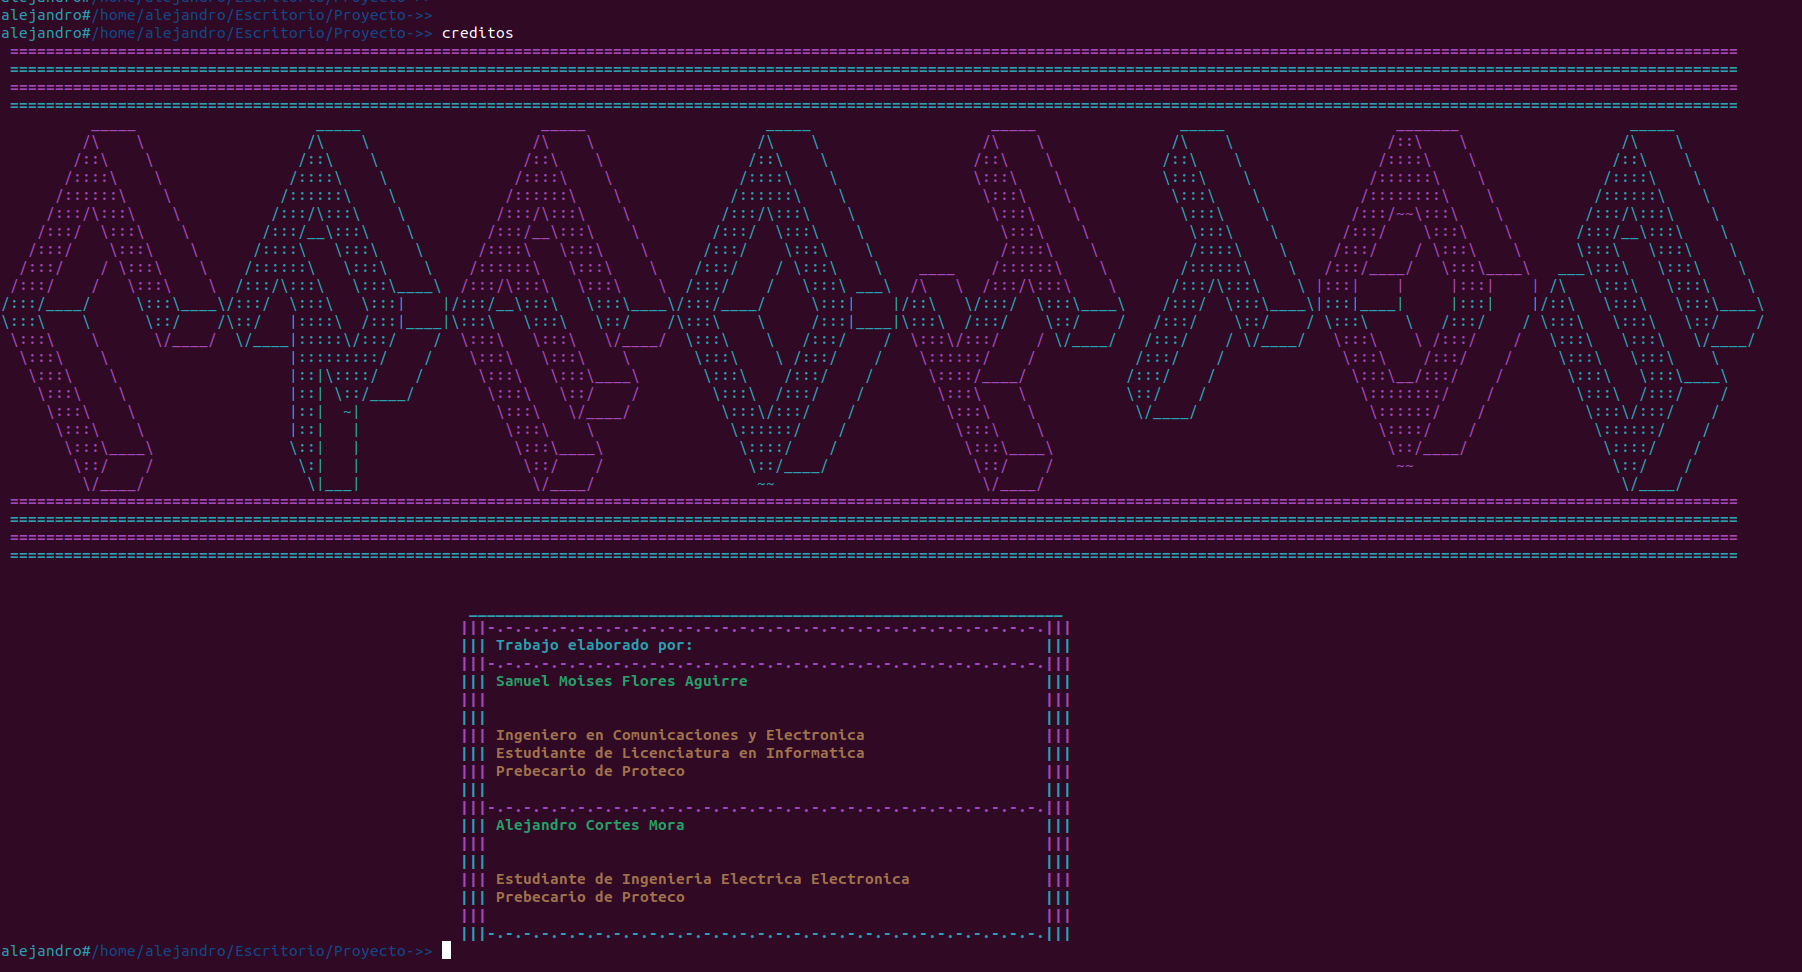
\includegraphics[width=1\textwidth]{capturaCreditos.png}
\end{center}

\vspace{1cm}
\fontsize{12}{6}\selectfont
\textbf{}

Muestra los creditos de los autores de esta terminal, en un recuadro dando la ocupacion de cada uno de ellos. 

\newpage

\subsection{Terminal}
\fontsize{9}{4}\selectfont
\begin{minted} [language=bash]{sh}


#!/bin/bash


echo ""
echo ""

echo -e "  \e[33m_________\e[0m\e[31m ___ ______________\e[0m\e[33m.____    .____      \e[0m"
echo -e " \e[33m/   _____/\e[0m\e[31m/   |   \_   _____/\e[0m\e[33m|    |   |    |     \e[0m"
echo -e " \e[33m\_____   \\e[0m\e[31m/    ~    \    __)_ \e[0m\e[33m|    |   |    |     \e[0m"
echo -e " \e[33m/        \ \e[0m\e[31m    Y    /        \\e[0m\e[33m|    |___|    |___  \e[0m"
echo -e "\e[33m/_______  /\e[0m\e[31m\___|_  /_______  /\e[0m\e[33m|_______ \_______ \ \e[0m"
echo -e "     \e[33m   \/       \e[0m\e[31m\/        \/       \e[0m\e[33m  \/       \/ \e[0m"
echo ""
echo ""


function login(){

	trap 'echo "No puedes ejecutar ese comando para salir"' SIGINT
	trap 'echo "No puedes ejecutar ese comando para salir"' SIGTSTP 
	comando='nosalir'
	creditos=(./creditos.sh)
	fecha=(./fecha.sh)
	ayuda=(./ayuda.sh)
	gato=(./game_gato.sh)
	infosis=(./infosis.sh)
	buscar=(./buscar.sh)
	reproductor=(./reproductor.sh)

	while [ "$comando" != 'salir' ]
	do
		echo -e -n "\e[36m$username#\e[0m\e[34m$PWD->> \e[0m" 
			
		read comando
		
		case $comando in
			
			creditos)
				$creditos
			;;
			
			fecha)
				$fecha
			;;
			
			gato)
				$gato
			;;
			
			ayuda)
				$ayuda
			;;
			
			infosis)
				$infosis
			;;
			
			buscar)
				$buscar
			;;
			
			reproductor)
				$reproductor
			;;
		esac
		
	done


}




error=2
while [ $error != 0 ] 
do
	echo ""
	echo -e -n "\e[33mIngrese su nombre de usuario: \e[0m"
	read username
	echo ""
	
	echo -e -n "\e[33mIngrese su contraseña: \e[0m"
	read -s password
	echo ""

	if id "$username" >/dev/null 2>&1; 
	then
		echo "Usuario correcto"
		#contrasena=$(sudo grep $username /etc/shadow | cut -d':' -f2)
		#if [[ $(echo "$password" | openssl passwd -1 -stdin) = "$contrasena" ]];
		#then
			echo "Puedes ingresar, bienvenido $username"
    			login
    			exit 0
    		#else
    		#	echo "Contraseña incorrecta"
    		#	error=$((error - 1))
    		#fi
	else
		echo ""
		echo "Usuario incorrecto"
		echo "Intenta de nuevo"
		error=$((error - 1))

	fi
	echo ""

done

if [ $error -eq 0 ];
then
	echo ""
	echo "No puedes ingresar"
	exit 1
fi



\end{minted}
\begin{center}
    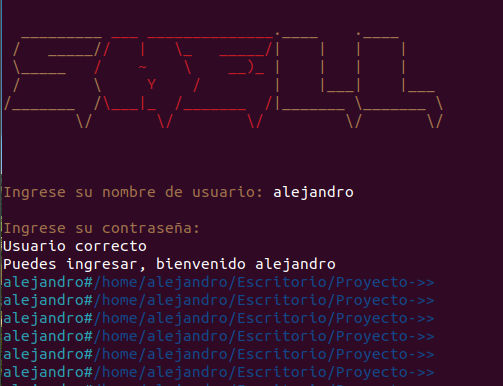
\includegraphics[width=0.8\textwidth]{capturaTerminal.png}
\end{center}

\vspace{1cm}
\fontsize{12}{6}\selectfont
\textbf{}

Esta terminal pide un logeo del usuario, si se encuentra dentro del sistema operativo, permitirá ingresar a la terminal, muestra el ususario y la ruta donde se encuentra posicionado. El usuario al ingresar un comando erronéo o no exitente no lo sacara, permitirá que se quede ahi hasta que se ejecute el comando salir. En caso de que el usuario falle al ingresar sus credenciales, solo tendra 3 oportunidades de intentarlo, ya que de lo contrario, se terminara abruptamente.



\section{Conclusiones}
\vspace{0.7cm}

\fontsize{14}{8}\selectfont

\textbf{Alejandro Cortés Mora}
Se programo la terminal, haciendo uso de los temas vistos durante el curso, y de material externo, como lo son investigacones, documentación relacionada, videos y paginas web de interés. Se utilizó lógica de programación para implementar los codigos, usando como referencia el lenguaje de programación C. Es importante destacar que, el hecho de crear los diferentes comandos realmente cumplio el propósito, mejorando, aplicando y comprendiendo los conocimientos adquiridos durante el curso, y el parendizaje integral que esto conlleva, mejorando asi, no solo en conocimientos del sistema operativo GU/Linux, como funciona y como se distribuye, sino, mejorando en lógica de programación, resolución de problemas y pensamiento critíco. Se espera no dejar el proyecto aqui, subuendo este en un repositorio de gitHub, que pueda ser útil a la comunidad que incursiona en este mundo de Linux, siendo asi un parteaguas para cualquier persona, y sobre todo, para nosotros, ya que aqui comienza el verdadero aprendizaje y el crecimiento.  

\vspace{0.5cm}
\textbf{Samuel Moíses Flores Aguirre}
Con este proyecto podemos concluir que a traves de los conocimientos adquiridos en el curso recibido por parte de los compañeros de Proteco, se pudo mejorar las habilidades en el sistema operativo Linux. Al realizar esta terminal de comandos, que a su vez fue compuesta por un comando infosis, un juego interactivo, un reproductor mp3, asi como los comandos de ayuda y buscar, se mejoro la capacidad de abstraccion, asi como la logica para su diseño e implementacion. En lo personal me quedo con el deseo de seguir aprendiendo y mejorando aun mas mis habilidades en el SO Linux.
De acuerdo a todo lo realizado, se pudo lograr el objetivo que se tenia planteado, que era construir una terminal de acuerdo a ciertas especificaciones requeridas. 

\end{document}


